\begin{definition}
    Krzywa eliptyczna to zbiór rozwiązań \( (x, y) \) w pewnym ciele \( \mathbb{F} \) równania:
    \[
        y^2 + a_1xy + a_2y = x^3 + b_1x^2 + b_2x + b_3,
    \]
    które można sprowadzić do postaci Weierstrassa:
    \[
        y^2 = x^3 + ax + b
    \]
\end{definition}

Chcemy, żeby krzywa była ,,gładka'' (nie jak Rys.~\ref{fig:elliptic_curves}d) i nie miała ,,ostrza'' (nie jak Rys.~\ref{fig:elliptic_curves}c), czyli formalnie, żeby wyznacznik krzywej \( \Delta = 4a^3 + 27b^2 \) był różny od 0.

\begin{figure}[H]
\centering
    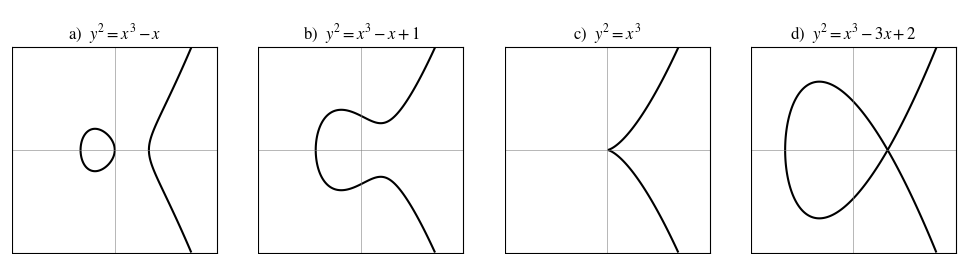
\includegraphics[width=0.8\textwidth]{img/elliptic_curves}
    \caption{Możliwe kształty krzywych eliptycznych w \( \real^2 \)}
    \label{fig:elliptic_curves}
\end{figure}

\subsection{Działania na krzywej eliptycznej}
Jeśli punkt \( P = (x, y) \) leży na krzywej eliptycznej, to \( -P = (x, -y) \) również.
Jeśli \( P \) i \( Q \) są punktami na krzywej eliptycznej, to prosta \( PQ \) przecina krzywą jeszcze w jednym punkcie \( R \).
Ustalamy, że \( P + Q + R = O \), gdzie \( O \) jest sztucznym punktem, który leży ,,w nieskończoności''.

\begin{figure}[H]
\centering
    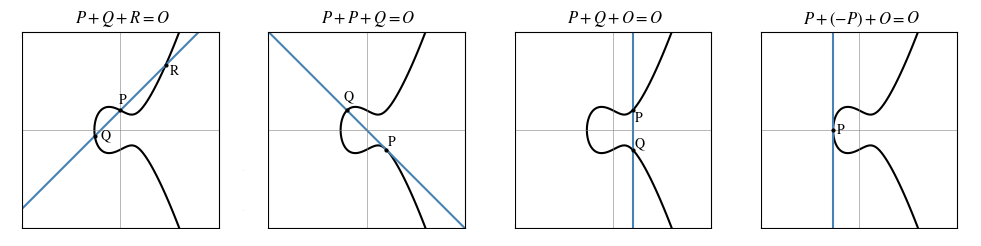
\includegraphics[width=0.8\textwidth]{img/elliptic_curves_lines}
    \caption{Możliwe przecięcia prostej z krzywą eliptyczną}
    \label{fig:elliptic_lines}
\end{figure}

Jeżeli \( Q = P \), traktujemy punkt \( P \) trochę jak podwójny pierwiastek wielomianu, który odbija się od osi, nie przecinając jej.
Za prostą \( PQ \) przyjmujemy wtedy styczną do krzywej w \( P \) (Rys.~\ref{fig:elliptic_lines}b).

Jeżeli \( Q = -P \), przyjmujemy, że \( P + Q = P + (-P) = O \) oraz \(P + O = P \) (Rys.~\ref{fig:elliptic_lines}c).

Podsumowując:
\begin{definition}[Dodawanie]
    Jeśli \( P \), \( Q \) są punktami na krzywej eliptycznej, to punkt \( R \) przecięcia prostej \( PQ \) z krzywą daje wynik dodawania \( P + Q = -R \).
    Jeśli prosta \( PQ \) nie przecina krzywej w dodatkowym punkcie, to \( P + Q = O \).
\end{definition}

Ponieważ mnożenie wymaga stałej liczby operacji, to dla dowolnego punktu \( P \) oraz liczby \( k \) można obliczyć \( k \cdot P \) w \( \bigO(\log k) \) operacjach arytmetycznych w ciele, stosując coś w rodzaju szybkiego potęgowania.

\subsection{Grupa krzywej eliptycznej}
Dodawanie punktów na krzywej jest przemienne i (co nieoczywiste) łączne, więc otrzymujemy grupę przemienną.

Najczęściej używa się krzywych:
\begin{itemize}
    \item nad \( \integer_p \), gdzie \( p \) jest dużą liczbą pierwszą,
    \item nad ciałem \( \text{GF}(2^s) \).
\end{itemize}

\begin{theorem}
    Niech \( \mathbb{F} \) będzie ciałem, \( \abs{\mathbb{F}} = q \) oraz niech \( E \) będzie grupą dla pewnej krzywej eliptycznej nad \( \mathbb{F} \). Grupa \( E \) jest albo grupą cykliczną, albo produktem dwóch grup cyklicznych.
\end{theorem}
Pozostawiamy to twierdzenie bez dowodu.

Rozmiar grupy \( \abs{E} \) może być rozumiany jako liczba rozwiązań równania opisującego krzywą.
Dla każdego \( x \in \mathbb{F} \) wartość \( x^3 + ax + b \) jest resztą kwadratową z prawdopodobieństwem \( \frac{1}{2} \). Jeśli uda się trafić, to otrzymamy dwa możliwe \( y \), więc punktów powinno być blisko \( q \).

Dokładnie, z twierdzenie Hassego: 
\[
    q - 2\sqrt{q} + 1 \leq \abs{E} \leq q + 2\sqrt{q} + 1
\]